%! Author = Luis
%! Date = 26.01.2024


\chapter{Planung und Entwurf}\label{ch:planung-und-entwurf}


\section{Organisation}\label{sec:organisation}
Da ich nicht im Team arbeite, ist die Organisation trivial.
Um einen groben und flexiblen Plan zu haben orientierte ich mich an Scrum und verwendete einen Backlog mit User Storys.
Eine unterteilung in Product Backlog und Sprint Backlog war hier nicht angebracht.
Die Eintr{"a}ge (User Storys) im Backlog sind nicht technisch, sondern fachlich.
Sie folgen einem einheitlichen Schema:
\begin{center}
    Als ``Rolle'' m{"o}chte ich ``Ziel/Wunsch'' (, um ``Nutzen'').
\end{center}

\subsection{User Rollen}\label{subsec:user-rollen}
Ich verwende drei einfache Rollen, um Personen zu klassifizieren, die mit der Anwendung interagieren:
\begin{itemize}
    \item Visitor - jemand der die Seite nur besucht.
    \item User - jemand der einen Account hat.
    \item Admin - jemand der die Seite verwaltet.
\end{itemize}

\subsection{User Storys}\label{subsec:user-storys}

\begin{CheckList}{Task}
    \Task{done}{Als Visitor m{"o}chte ich meine Ip-Adresse teilen, um sie auf einem andern Ger{"a}t abzurufen.}
    \Task{done}{Als Visitor m{"o}chte ich {"u}ber die Risiken des Teilens, informiert werden.}
    \Task{open}{Als Visitor m{"o}chte ich {"u}ber das Anlegen eines Users informiert werden.} %todo Texte auf Register Seite Fehlen.
    \Task{done}{Als Visitor m{"o}chte ich einen Accout Registirern, um User zu werden.}
    \Task{started}{Als Visitor m{"o}chte ich die App ohne Cookies nutzen k{"o}nnen.}
    \Task{done}{Als Admin m{"o}chte ich eine requirements.txt.}
    \Task{started}{Als User m{"o}chte ich eine Liste aller meiner IPs sehen und diese Sortieren k{"o}nnen.}
    \Task{done}{Als User m{"o}chte ich meine Ip Passwort gesch{"u}tzt teilen.}
    \Task{started}{Als User m{"o}chte ich sehen wann die Ip geteilt wurde.}
    \Task{open}{Als User m{"o}chte ich leicht herausbekommen wie ich die API verwenden kann. (Immer hinweise wie ich die Informationen mit der API abrufen k{"o}nnte?!)}
    \Task{done}{Als User m{"o}chte ich mich anmelden.}
    \Task{done}{Als User m{"o}chte ich meinen account L{"o}schen k{"o}nnen.}
    \Task{done}{Als User m{"o}chte ich meinen Passwort {"a}ndern k{"o}nnen.}
    \Task{done}{Als User m{"o}chte ich meinen Remember Cookie einstellen k{"o}nnen.}
    \Task{done}{Als User m{"o}chte ich meine Token invalidieren k{"o}nnen.}
    \Task{dropped}{Als User m{"o}chte ich meine Adressen ver{"o}ffentlichen k{"o}nnen.} % -> kein ver{"o}ffentlichen beliebiger Inhalte.
    \Task{done}{Als User m{"o}chte ich {"o}ffentliche Ips importieren/namen.}
    \Task{done}{Als User m{"o}chte ich Adressen manuell eingeben k{"o}nnen.}
    \Task{open}{Als User Ipv4 und Ipv6 (evtl. onion-url) validierung.}
    \Task{open}{Als User m{"o}chte ich meine Adressen in Gruppen teilen k{"o}nnen.}
    \Task{open}{Als User m{"o}chte meine Aderssen als QR-Code angezeigt bekommen.}
    \Task{open}{Als Admin m{"o}chte ich eine Firewall.}
    \Task{open}{Als Admin m{"o}chte ich AGB und Datenschutzerkl{"a}rung haben.}
    \Task{open}{Als Admin m{"o}chte ich IPs GEO blocken bzw. differrenzeiren.}
    \Task{done}{Als User m{"o}chte meine Aderssen in Echtzeit aktualisiert haben.}
    \Task{started}{Als Admin m{"o}chte Rate Limits auf den Routen.}
    \Task{dropped}{Als User m{"o}chte ich einen Cookie banner.}
    \Task{open}{Als Visitor m{"o}chte ich keine Cookies.}
    \Task{open}{Als User m{"o}chte ich {"u}ber E-Mail informiert werden k{"o}nnen wenn der Service nicht verf{"u}gbar ist oder sich {"a}ndert.}
    \Task{unclear}{Als User m{"o}chte ich einen Reverse VPN {"o}ffnen k{"o}nnen.}
    \Task{open}{Als User m{"o}chte ich mein Adressen einfach mit Api abrufen k{"o}nnen.} % Tokens
    \Task{open}{Als User und Visitor m{"o}chte ich ein {"u}bersichtliches Interface.}
    \begin{CheckList}{Task}
        \Task{open}{Kenntlich machen von Public und Private}
        \Task{open}{Als User und Visitor m{"o}chte ich Mehrsprachigkeint. (Englisch und Deutsch evtl. weitere)}
        \Task{done}{Als User und Visitor m{"o}chte ich durch klicken Adressen und Namen Kopieren.}
        \Task{open}{Teilen durch klicken auf IP ist unklar. -> Share Icon?!}
        \Task{open}{Als User und Visitor m{"o}chte ich Tooltips.}
    \end{CheckList}
    \Task{open}{Als Visitor m{"o}chte ich das es Schwer oder unm{"o}glich ist einen Link zu erstellen der automatisch/unfreiwilliges meine Adresse teilt.}
    \Task{unclear}{Als Admin m{"o}chte ich Datenbank Migrationen.}
    \Task{done}{Als Admin m{"o}chte ich Blueprints.}
    \Task{open}{Als Admin m{"o}chte ich Logging, um Angirffe und Fehler zu erkennen.}
\end{CheckList}


\section{Frameworks und Entwicklungsumgebung}\label{sec:frameworks-und-entwicklungsumgebung}
Ich verwende Flask als Framework und programmiere in PyCharm Professional 2023.
Mein verwalte mein Python Environment und meine Pakete mit Anaconda\cite{anaconda}.
Die verwendete Python Version ist 3.11.5.
Zur Versionierung verwende ich git und GitHub.
Die verwendeten Bibliotheken und deren Versionen finden sich im environment.yml oder im requirements.txt.
Hier eine Kure Übersicht:

\begin{itemize}
    \item Flask
    \begin{itemize}
        \item APScheduler
        \item Bcrypt
        \item Limiter
        \item Login
        \item SocketIO
        \item SQLAlchemy
        \item WTF
    \end{itemize}
    \item NumPy
    \item OpenCV
    \item qrcode
    \item Pillow
    \item Requests
    \item PyJWT
    \item urllib3
\end{itemize}


\section{Datenbankstruktur}\label{sec:datenbankstruktur}
Die Datenbank ist relativ simple es gibt eine User- und eine Address-Tabelle.
%user only one to zero or more shared-addresses
Es gelten folgende Abh{"a}ngigkeiten:

\begin{align}
    id ~ &\dot \rightarrow ~ passwort \\
    id ~ &\dot \rightarrow ~ remember \\
    id ~ &\dot \leftrightarrow ~ alternative\_id \\
    id ~ &\dot \leftrightarrow ~ name \\
    id, device\_name ~ &\dot \rightarrow ~ address \\
    id, device\_name ~ &\dot \rightarrow ~ last\_updated
\end{align}


\begin{figure}[h]
    \centering
    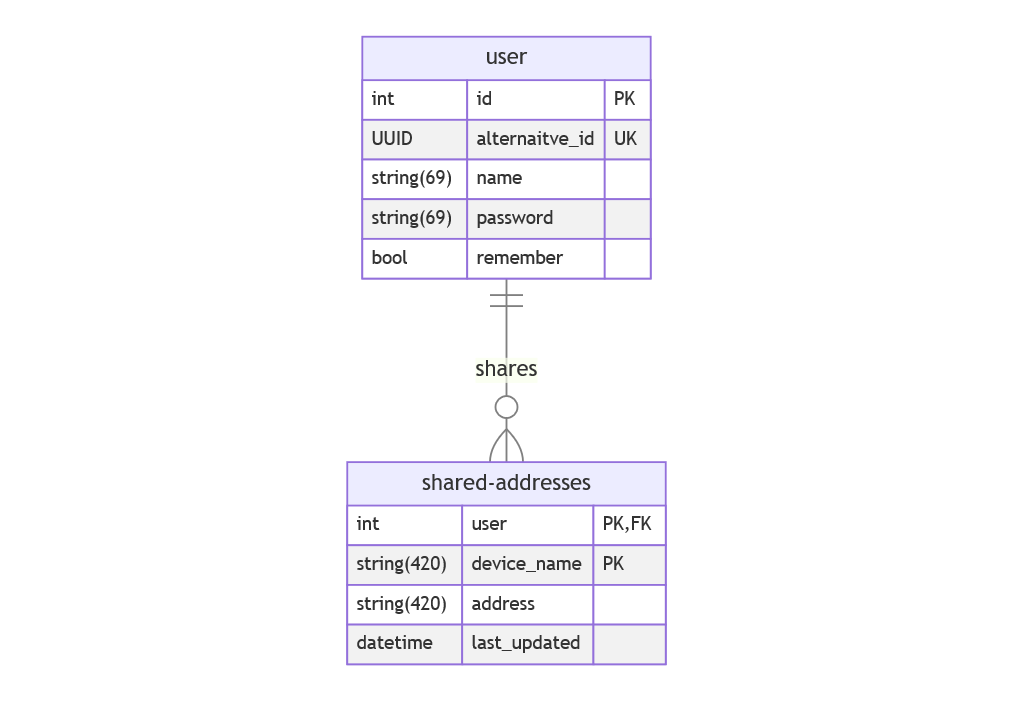
\includegraphics[width=\textwidth]{db}
    \caption{Entity-Relationship-Modell der DB}
    \label{fig: db}
\end{figure}



